%!TEX root = ../main.tex
%%%%%%%%%%%%%%%%%%%%%%%%%%%%%%%%%%%%%%%%%%
%
%LEZIONE 19/04/2016 - OTTAVA SETTIMANA (1)
%
%%%%%%%%%%%%%%%%%%%%%%%%%%%%%%%%%%%%%%%%%%
\chapter{Forme differenziali}
%%%%%%%%%%%%%%
%INTRODUZIONE%
%%%%%%%%%%%%%%
\section{Introduzione}

\begin{defn}{Forma differenziale}{formaDifferenziale}\index{Forma differenziale}
	Sia \(\Omega\subseteq \R^n\) aperto.
	Una \emph{forma differenziale} in \(\Omega\) è una funzione continua
	\[
		F\colon \Omega \to \big(\R^n\big)^*.
	\]
\end{defn}

\begin{defn}{Base duale}{baseDuale}\index{Base duale}
	Presa \(\{e_1,\ldots,e_n\}\) la base canonica di \(\R^n\), la base duale
	\[
		\{\dd x_1,\ldots, \dd x_n\},
	\]
	è una base di \(\big(\R^n\big)^*\) univocamente identificata dalla seguente relazione
	\[
		\dd x_i (e_j) = \d_{i\,j}.
	\]
\end{defn}

\begin{oss}
	Con \(\dd x_i\) abbiamo quindi definito un operatore lineare di \(\R^n\) che al generico vettore \(h\in\R^n\) associa la sua componente \(i\)-esima \(h_i\).
\end{oss}

\begin{defn}{Integrale di una forma differenziale lungo una curva}{integraleFormaDifferenziale}\index{Integrale!di una forma differenziale}
	Sia \(\Omega\subseteq\R^n\) un aperto e sia \(F\colon \Omega \to \big(\R^n\big)^*\) una forma differenziale.
	Sia \(\g\colon [a,b]\to\R^n\) una curva di classe \(C^1\) su \([a,b]\) compatto.
	Definiamo l'integrale di \(F\) lungo \(\g\) come
	\[
		\int\limits_\g F = \int_a^b F\big(\g(t)\big) \dot{\g}(t)\,\dd t.
	\]
\end{defn}

\begin{oss}
	Nell'ultima uguaglianza, le dimensione dei termini sono ben definite, infatti
	\[
		F\big(\g(t)\big) \in \big(\R^n\big)^* \qquad\text{e}\qquad \dot{\g}(t)\in\R^n.
	\]
\end{oss}

\begin{oss}
	Il termine \(\dot{\g}(t)\) indica il versore tangente alla curva orientato nella direzione di spostamento di \(\g\).
\end{oss}

\begin{oss}
	Questa definizione corrisponde, in fisica, alla definizione di lavoro svolto per passare da \(\g(a)\) a \(\g(b)\) sotto l'azione del campo di forze \(F\).
\end{oss}

\begin{oss}
	Una scrittura equivalente è la seguente:
	\[
		\int\limits_\g F = \int_a^b \sum_{i=1}^n F_i \big(\g(t)\big) \dot{\g}_i(t)\,\dd t.
	\]
\end{oss}

\begin{ese}
	Consideriamo la seguente forma differenziale
	\[
		F\colon \R^2\setminus\{(0,0)\} \to \big(\R^2\big)^*, 	\begin{pmatrix}
			x \\
			y
		\end{pmatrix}
		\mapsto \left( -\frac{y}{x^2+y^2},\frac{x}{x^2+y^2} \right) = -\frac{y}{x^2+y^2}\dd x + \frac{x}{x^2+y^2}\dd y.
	\]
	E la curva che parametrizza la circonferenza
	\[
		\g\colon [0,2\p] \to \R^2, t\mapsto \begin{pmatrix}
			R \cos t \\
			R \sin t
		\end{pmatrix}
	\]
	Calcoliamo l'integrale di \(F\) lungo \(\g\):
	\[
		\begin{split}
			\int\limits_\g F & = \int_0^{2\p} \left( -\frac{R\sin t}{R^2}, \frac{R\cos t}{R^2} \right) \begin{pmatrix}-R\sin t\\R\cos t\end{pmatrix}\,\dd t\\
			& = \int_0^{2\p} \sin^2(t)+\cos^2(t)\,\dd t\\
			& = \int_0^{2\p} \dd t = 2\p.
		\end{split}
	\]
	Dal risultato ci viene il sospetto che \(F\) sia la forma differenziale che conta i giri attorno all'origine.
\end{ese}

\begin{defn}{Potenziale di una forma differenziale}{pontenzialeFormaDifferenziale}\index{Potenziale}
	Sia \(\Omega\subseteq\R^n\) aperto e sia \(F\colon \Omega\to \big(\R^n\big)^*\) una forma differenziale.
	\(V\in C^1(\Omega,\R)\) si dice \emph{potenziale} di \(F\) se
	\[
		F(x) = V'(x),\,\fa x\in \Omega.
	\]
\end{defn}

\begin{notz}
	Scriveremo \(\dd V(x)=V'(x)\).
\end{notz}

\begin{defn}{Forma differenziale esatta}{formaDifferenzialeEsatta}\index{Forma differenziale!esatta}
	Sia \(\Omega\subseteq\R^n\) aperto e sia \(F\colon \Omega\to \big(\R^n\big)^*\) una forma differenziale.
	\(F\) si definisce \emph{forma differenziale esatta} se esiste un potenziale \(V\in C^1(\Omega,\R)\) di \(F\).
\end{defn}

\begin{oss}
	Se \(V\in C^1(\Omega,\R)\) è un potenziale di \(F\), allora \(V'\) è un elemento del duale di \(R^n\), ovvero
	\[
		V'(x) = \big(\pd_1 V(x),\ldots,\pd_n V(x)\big) = \pd_1 V(x)\,\dd x_1 + \ldots + \pd_n V(x)\,\dd x_n.
	\]
	In particolare, se \(\g\colon [a,b]\to \R^n\) è una curva di classe \(C^1\), avremo
	\[
		\begin{split}
			\int\limits_\g F = \int\limits_\g V' & = \int_a^b \big(\pd_1 V(x),\ldots,\pd_n V(x)\big)|_{\g(t)} \begin{pmatrix}\dot{\g}_1(t)\\\vdots\\\dot{\g}_n(t)\end{pmatrix}\,\dd t\graffito{applicando prima la regola della catena e poi il TFC}\\
			& = \int_a^b \frac{\dd}{\dd t} V\big(\g(t)\big)\,\dd t\\
			& = V\big(\g(b)\big) - V\big(\g(a)\big).
		\end{split}
	\]
\end{oss}

\begin{teor}{Indipendenza dalla parametrizzazione}{indipendenzaParametrizzazioneForme}
	Siano \(F\colon \Omega \to \big(\R^n\big)^*\) una forma differenziale e \(\g\colon [a,b]\to \Omega\) una curva di classe \(C^1\).
	Sia \(\y\colon [c,d]\to [a,b]\) di classe \(C^1\).
	Allora
	\begin{itemize}
		\item Se \(\y(c)=a\) e \(\y(d)=b \implies \displaystyle \int\limits_{\g\circ \y} F = \int\limits_\g F\).
		\item Se \(\y(c)=b\) e \(\y(d)=a \implies \displaystyle \int\limits_{\g\circ \y} F = -\int\limits_\g F\).
	\end{itemize}
\end{teor}

\begin{proof}
	Mostriamo il caso in cui \(\y(c)=a\) e \(\y(d)=b\), il secondo caso è del tutto analogo.

	Applicando la definizione avremo
	\[
		\begin{split}
			\int\limits_{\g\circ \y} F & = \int_c^d F\big(\g\circ \y(t)\big) \frac{\dd}{\dd t}\g\circ \y(t)\,\dd t\graffito{regola della catena}\\
			& = \int_c^d F\big(\g\circ \y(t)\big) \dot{\g}|_{\y(t)} \y'(t)\,\dd t\graffito{pongo \(s=\y(t)\)}\\
			& = \int_a^b F\big(\g(s)\big)\dot{\g}(s)\,\dd s\\
			& = \int\limits_\g F.\qedhere
		\end{split}
	\]
\end{proof}
%%%%%%%%%%%
%PULL-BACK%
%%%%%%%%%%
\section{Pull-back}

Prima di addentrarci nel problema del pull-back, vorremmo poter definire le seguenti relazioni
\[
	\int\limits_{-\g} F = -\int\limits_\g F \qquad\text{e}\qquad \int\limits_{\mathclap{\g_1+\g_2}} F = \int\limits_{\g_1} F + \int\limits_{\g_2} F,
\]
facendo attenzione che con \(-\g\) non si intende la funzione che associa ad ogni \(t\) il valore \(-\g(t)\) ma bensì la curva che percorre \(\g\) nel verso contrario.\graffito{analogamente con \(\g_1+\g_2\) si fa riferimento alla curva che percorre prima \(\g_1\) e poi \(\g_2\)}

Per dare una veste rigorosa a questa definizione osserviamo che \(\g\) è un elemento del duale delle forme differenziali.
Infatti, fissato \(\g\), trovo
\[
	A_\g \colon F \mapsto \int\limits_\g F,
\]
ovvero l'operatore lineare che manda le forme differenziali in \(\R\).
Ora, in quanto operatore lineare,
\[
	A_\g(a\,F_1+b\,F_2) = \int\limits_\g (a\,F_1+b\,F_2) = a\int\limits_\g F_1 + b\int\limits_\g F_2 = a\,A_\g(F_1)+b\,A_\g(F_2).
\]
Quindi con \(\g_1+\g_2\) o \(-\g\) si intende rispettivamente \(A_{\g_1}+A_{\g_2}\) o \(-A_\g\), ovvero un'operazione fra operatori lineari.

Introduciamo quindi il problema del pull-back:
data una forma differenziale \(F\) su \(\Omega\) e un diffeomorfismo \(g\colon \Omega'\to \Omega\), vorremmo poter definire una forma differenziale \(\tilde{F}\) su \(\Omega'\) tale che, per ogni curva \(\g\) su \(\Omega'\) valga
\[
	\int\limits_\g \tilde{F} = \int\limits_{\mathclap{g\circ \g}} F.
\]

\begin{defn}{Pull-back}{pull-back}\index{Pull-back}
	Siano \(\Omega,\Omega'\) due aperti di \(\R^n\) e sia \(g\colon \Omega' \to \Omega\) un diffeomorfismo.
	Presa una forma differenziale \(F\) su \(\Omega\), si definisce il \emph{pull-back} di \(F\) come
	\[
		\tilde{F}\colon \Omega' \to \big(\R^n\big)^*, \tilde{F}(x) = F\big(g(x)\big)g'(x).
	\]
\end{defn}

\begin{teor}{Invarianza dell'integrale tramite pull-back}{invarianzaPull-back}
	Siano \(\Omega,\Omega'\) due aperti di \(R^n\) e sia \(g\colon \Omega'\to \Omega\) un diffeomorfismo.
	Sia \(F\colon \Omega\to \big(\R^n\big)^*\) una forma linare e sia \(\tilde{F}\colon \Omega' \to \big(\R^n\big)^*\) il suo pull-back.
	Allora
	\[
		\int\limits_{\mathclap{g\circ \g}} F = \int\limits_\g \tilde{F},
	\]
	per ogni curva \(\g\) su \(\Omega'\) di classe \(C^1\).
\end{teor}

\begin{proof}
	Sia \(\g\colon [a,b] \to \Omega'\) una curva di classe \(C^1\).
	Avremo
	\[
		\int\limits_{\mathclap{g\circ \g}} F = \int_a^b F\big(g\circ \g(t)\big) \frac{\dd}{\dd t}g\circ \g(t)\,\dd t = \int_a^b F\big(g\circ \g(t)\big) g'|_{\g(t)} \dot{\g}(t)\dd t.
	\]
	Per definizione il pull-back di \(F\) è definito come \(\tilde{F}(x) = F\big(g(x)\big)g'(x)\).
	Quindi
	\[
		\int_a^b F\big(g\circ \g(t)\big) g'|_{\g(t)} \dot{\g}(t)\dd t = \int_a^b \tilde{F}\big(\g(t)\big)\dot{\g}(t)\,\dd t = \int\limits_\g \tilde{F}.\qedhere
	\]
\end{proof}

\begin{oss}
	Se \(F\) è una forma differenziale esatta, \(F=\dd V\), allora \(\tilde{F}=\dd \tilde{V}\) con \(\tilde{V} = V\circ g\).
	Infatti
	\[
		\dd\tilde{V} = \dd V|_{g(x)} g'(x) = F\big(g(x)\big)g'(x) = \tilde{F}(x).
	\]
\end{oss}

\begin{ese}
	Consideriamo nuovamente l'esempio del paragrafo precedente.
	Sia \(g\) il diffeomorfismo delle coordinate polari definito al di fuori dell'asse positiva delle \(x\):
	\[
		g\colon (0,+\infty) \times (0,2\p) \to \R^2\setminus\Set{(x,0) | x\ge 0}, \begin{pmatrix}\r\\\q\end{pmatrix} \mapsto \begin{pmatrix}\r\cos\q\\\r\sin\q\end{pmatrix}
	\]
	Ricordiamo che la forma differenziale era definita come
	\[
		F\colon \R^2 \setminus\Set{(x,0) | x\ge 0} \to \big(\R^2\big)^*, \begin{pmatrix}x\\y\end{pmatrix} \mapsto \left( -\frac{y}{x^2+y^2},\frac{x}{x^2+y^2} \right).
	\]
	Per definizione il pull-back di \(F\) tramite \(g\) sarà:
	\[
		\begin{split}
			\tilde{F} \begin{pmatrix}\r\\\q\end{pmatrix} & = F \begin{pmatrix}\r\cos\q\\\r\sin\q\end{pmatrix} \begin{pmatrix} \cos\q & -\r\sin\q\\ \sin\q & \r\cos\q\end{pmatrix} = \left( -\frac{1}{\r}\sin\q, \frac{1}{\r}\cos\q \right) \begin{pmatrix}\cos\q & -\r\sin\q\\\sin\q & \r\cos\q\end{pmatrix}\\
			& = (0,1) = \dd\q,
		\end{split}
	\]
	che è quindi una forma differenziale esatta.
\end{ese}
%%%%%%%%%%%%%%%%%%%%%%%%%%%%%%%%%%%%%%%%%%
%
%LEZIONE 20/04/2016 - OTTAVA SETTIMANA (2)
%
%%%%%%%%%%%%%%%%%%%%%%%%%%%%%%%%%%%%%%%%%%
%%%%%%%%%%%%%%
%FORME CHIUSE%
%%%%%%%%%%%%%%
\section{Forme chiuse}

\begin{defn}{Forma differenziale chiusa}{formaDifferenzialeChiusa}\index{Forma differenziale!chiusa}
	Sia \(F\) una forma differenziale di classe \(C^1\).
	\(F\) si definisce \emph{chiusa} se ha le derivate miste uguali, ovvero
	\[
		\pd_j F_i(x) = \pd_i F_j(x),\,\fa i,j.
	\]
\end{defn}

\begin{oss}
	Se \(F=V'\) con \(V\in C^2\) allora \(F\) è chiusa.
	Infatti avremo
	\[
		F(x) = F_1(x)\,\dd x_1+ \ldots + F_n(x)\,\dd x_n = \pd_1 V(x)\,\dd x_1 + \ldots + \pd_n V(x).
	\]
	Ma \(V\in C^2(\Omega)\), quindi per il lemma di Schwarz
	\[
		\pd_j F_i(x) = \pd_i F_j(x).
	\]
\end{oss}

\begin{oss}
	In generale il viceversa è falso, infatti
	\[
		F\colon \begin{pmatrix}x\\y\end{pmatrix} \mapsto -\frac{y}{x^2+y^2}\,\dd x + \frac{x}{x^2+y^2}\,\dd y,
	\]
	ha \(\pd_y F_x= \pd_x F_y\) ma abbiamo già osservato che su \(\R^2\setminus\{(0,0)\}\) non è esatta.
\end{oss}

\begin{teor}{Caratterizzazione delle forme esatte}{caratterizzazioneFormeEsatte}
	Sia \(\Omega\subseteq \R^n\) un aperto e sia \(F\colon \Omega \to \big(\R^n\big)^*\) una forma differenziale.
	Allora le proprietà seguenti si equivalgono:
	\begin{enumerate}
		\item \(F\) è una forma esatta.
		\item Per ogni curva chiusa \(\g\) in \(\Omega\) si ha \(\displaystyle \int\limits_\g F=0\).
		\item Se \(\g_1\) e \(\g_2\) sono curve in \(\Omega\) aventi gli stessi estremi, si ha \(\displaystyle \int\limits_{\g_1} F = \int\limits_{\g_2} F\).
	\end{enumerate}
\end{teor}

\begin{proof}
	\graffito{\(1)\implies 2)\)}Supponiamo che \(F\) sia esatta, trovo quindi \(V\in C^1(\Omega,\R)\) tale che \(F=V'\).
	Quindi
	\[
		\int\limits_\g F = V\big(\g(b)\big) - V\big(\g(a)\big),
	\]
	dove \(\g\colon [a,b]\to \Omega\) è una curva di classe \(C^1\) con \(\g(b)=\g(a)\) in quanto chiusa.
	Per cui
	\[
		V\big(\g(b)\big) - V\big(\g(a)\big) = 0.
	\]
	\graffito{\(2)\implies 3)\)}Supponiamo che \(\g_1\colon [a,b] \to \Omega\) e \(\g_2\colon [c,d] \to \Omega\) siano curve di classe \(C^1\) con
	\[
		\g_1(a) = \g_2(c) \qquad\text{e}\qquad \g_1(b) = \g_2(d).
	\]
	Ora \(\g_1-\g_2\) sarà la curva che percorre prima \(\g_1\) e poi \(\g_2\) in senso opposto.
	In particolare il punto iniziale di \(\g_1-\g_2\) sarà \(\g_1(a)\) mentre il punto finale \(\g_2(c)\), che per ipotesi coincidono.
	Quindi \(\g_1-\g_2\) è una curva chiusa, per cui
	\[
		0 = \int\limits_{\mathclap{\g_1-\g_2}} F = \int\limits_{\g_1} F - \int\limits_{\g_2} F.
	\]
	\graffito{\(3)\implies 1)\)}Per dimostrare che \(F\) è una forma esatta devo esibirne una primitiva.
	Fisso \(x_0\in\Omega\) e definisco
	\[
		V(x) = \int\limits_\g F,
	\]
	dove \(\g\) è una qualunque curva tale che parte da \(x_0\) e arriva in \(x\).\graffito{sappiamo per ipotesi che l'integrale dipende solo dagli estremi della curva}
	Vogliamo dimostrare che \(V'=F\).
	Per farlo mi basta verificare che \(\pd_{x_1}V = F_1, \ldots, \pd_{x_n}V = F_n\); in tal caso \(V\) è differenziabile per il teorema del differenziale totale in quanto \(F\) è continua.
	Devo calcolare
	\[
		\frac{V(x+t\,e_i)-V(x)}{t}.
	\]
	Sia \(\g_1\colon [0,1] \to \Omega, s\mapsto x+t\,s\,e_i\).
	Quindi
	\[
		\begin{split}
			\frac{V(x+t\,e_i)-V(x)}{t} & = \frac{1}{t}\left[ \int\limits_{\g+\g_1}F-\int\limits_\g F \right] = \frac{1}{t}\int\limits_{\g_1} F\\
			& = \frac{1}{t} \int_0^1 \Big(F_1\big(\g_1(s)\big),\ldots,F_n\big(\g_1(s)\big)\Big) t \begin{pmatrix}0\\\vdots\\1\\\vdots\\0\end{pmatrix}\,\dd s\\
			& = \int_0^1 F_i\big(\g_1(s)\big)\,\dd s \xrightarrow{t\to 0} F_i(x),
		\end{split}
	\]
	dove il limite sotto integrale è rigoroso in quanto \(F\) è continua e \([0,1]\) è un compatto.
\end{proof}

\begin{ese}
	Consideriamo nuovamente la forma differenziale
	\[
		F\colon \R^2\setminus\{(0,0)\} \to \big(\R^2\big)^*, \begin{pmatrix}x\\y\end{pmatrix} \mapsto -\frac{y}{x^2+y^2}\,\dd x + \frac{x}{x^2+y^2}\,\dd y.
	\]
	Tale forma su \(\R^2\setminus\{(0,0)\}\) non è esatta infatti abbiamo mostrato in precedenza che, sulla curva parametrica della circonferenza, l'integrale non è nullo.
	D'altronde su \(\R^2\setminus\Set{(x,0) | x\ge 0}\) lo è, infatti abbiamo precedentemente mostrato che ha \(\dd \q\) come primitiva.

	Questo accade in quanto \(\q\colon S^1 \to \R\) non è ben definita su tutta \(S^1\), infatti \(\q(0)=\q(2\p)\).
\end{ese}

\begin{teor}{Lemma di Poincaré}{lemmaPoincaré}\index{Lemma!di Poincaré}
	Sia \(F\colon B_r(x_0) \to \big(\R^n\big)^*\) una forma differenziale di classe \(C^1\).
	Allora \(F\) è chiusa se e soltanto se \(F\) è esatta.
\end{teor}

\begin{proof}
	\graffito{\(\Leftarrow)\)}Abbiamo già osservato, definendo le curve chiuse, che se una forma esatta, è automaticamente chiusa per il lemma di Schwarz.

	\graffito{\(\Rightarrow)\)}Dimostriamolo che esiste una primitiva di \(F\) per \(n=2\), il caso generale è del tutto analogo.
	Definisco
	\[
		V(x,y) = \int\limits_{\mathclap{\g_x+\g_{(x,y)}}} F,
	\]
	dove
	\[
		\g_x\colon [0,x-x_0] \to B_r\big((x_0,y_0)\big), t\mapsto (x_0+t,y_0)
	\]
	e
	\[
		\g_{(x,y)}\colon [0,y-y_0] \to B_r\big((x_0,y_0)\big), t \mapsto (x,y_0+t).
	\]
	Supponiamo che \(F(x,y)=F_x\,\dd x+ F_y\,\dd y\).
	Quindi
	\[
		\begin{split}
			\int\limits_{\mathclap{\g_x+\g_{(x,y)}}} F & = \int_0^{x-x_0} \big(F_x(x_0+t,y_0),F_y (x_0+t,y_0)\big) \begin{pmatrix}1\\0\end{pmatrix}\,\dd t\\
			& + \int_0^{y-y_0} \big(F_x(x,y_0+t),F_y(x,y_0+t)\big) \begin{pmatrix}0\\1\end{pmatrix}\,\dd t\\
			& = \int_0^{x-x_0} F_x(x_0+t,y_0)\,\dd t + \int_0^{y-y_0} F_y(x,y_0+t)\,\dd t.
		\end{split}
	\]
	Quindi
	\[
		\pd_y V(x,y) = F_y(x,y),
	\]
	per il TFC.
	Mentre
	\[
		\begin{split}
			\pd_x V(x,y) & = F_x(x,y_0) + \int_0^{y-y_0} \pd_x F_y(x,y_0+t)\,\dd t\graffito{\(F\) è chiusa quindi posso scambiare la derivata}\\
			& = F_x(x,y_0) + \int_0^{y-y_0} \pd_y F_x(x,y_0+t)\,\dd t\\
			& = F_x(x,y_0) + \int_0^{y-y_0} \frac{\dd}{\dd t} F_x(x,y_0+t)\,\dd t\\
			& = F_x(x,y_0) + F_x(x,y_0+t)|_0^{y-y_0}\\
			& = F_x(x,y_0) + F_x(x,y) - F_x(x,y_0)\\
			& = F_x(x,y),
		\end{split}
	\]
	dove la derivata sotto integrale è rigorosa in quanto \(F\) è di classe \(C^1\) e \([0,y-y_0]\) è compatto.
\end{proof}

\begin{oss}
	Se \(F\) è definita su un aperto semplicemente connesso allora \(F\) è esatta su tutto l'aperto.
\end{oss}

\begin{ese}
	Calcoliamo l'integrale di \(w = x\,\dd y\) su
	\[
		\g\colon [0,2\p]\to \R^2, t\mapsto \begin{pmatrix}x_0+R\cos t\\x_0+R\sin t\end{pmatrix}.
	\]
	Per definizione
	\[
		\begin{split}
			\int\limits_\g w & = \int_0^{2\p} (x_0+R\cos t)R\cos t\,\dd t\\
			& = x_0\,R \int_0^{2\p} \cos t\,\dd t + R^2 \int_0^{2\p} \cos^2 t\,\dd t\\
			& = \frac{R^2}{2} \int_0^{2\p} 1+\cos 2t\,\dd t = R^2 \p.
		\end{split}
	\]
	Quindi \(w\) non è esatta. D'altronde non è chiusa, infatti
	\[
		w = 0\,\dd x+ x\,\dd y \qquad\text{e}\qquad \pd_y 0 = 0 \neq \pd_x x = 1.
	\]
\end{ese}
%%%%%%%%%%%%%%%%%%%%%%%%%%%%%%%%%%%%%%%%
%
%LEZIONE 26/04/2016 - NONA SETTIMANA (1)
%
%%%%%%%%%%%%%%%%%%%%%%%%%%%%%%%%%%%%%%%%
%%%%%%%%%%%%%%%%%%%
%TEOREMA DI STOKES%
%%%%%%%%%%%%%%%%%%%
\section{Teorema di Stokes}

Sappiamo che se \(\w=a(x,y)\,\dd x+b(x,y)\,\dd y\) è una forma differenziale chiusa e \(\g\) è una curva chiusa, allora
\[
	\int\limits_\g \w = 0.
\]
Ora se \(\g\) è il bordo di un aperto \(A\subset\R^2\) posso scrivere
\[
	0 = \int\limits_\g \w = \int\limits_A \big[\pd_x b(x,y)-\pd_y a(x,y)\big]\,\dd x\,\dd y.
\]
Questo è un fatto generale che può essere formalizzato attraverso il teorema di Gauss-Green che è un'applicazione del teorema di Stokes in \(\R^2\).

\begin{teor}{di Gauss-Green}{gaussGreen}\index{Teorema!di Gauss-Green}
	Sia \(\w=a(x,y)\,\dd x+b(x,y)\,\dd y\) una forma differenziale di classe \(C^1\) nell'aperto \(B\subseteq \R^2\) e sia \(A\subseteq B\) un aperto con \(\overline{A}\subseteq B\).
	Supponiamo che la frontiera di \(A\) sia costituita da un numero finito di curve regolari chiuse e disgiunte \(\g_1,\ldots,\g_n\).
	Supponiamo inoltre che tali curve siano orientate in modo da lasciarsi \(A\) alla propria sinistra.
	Allora
	\[
		\iint\limits_A \big[\pd_x b(x,y)-\pd_y a(x,y)\big]\,\dd x\,\dd y = \sum_{i=1}^n \int\limits_{\g_i} \w = \int\limits_{\g_1+\ldots+\g_n} \w = \int\limits_{\pd A} \w.
	\]
\end{teor}

\begin{proof}
	Mostriamo il caso in cui \(\Gamma = \pd A\) è una curva singola e \(A\) è normale rispetto a entrambi gli assi, ovvero
	\[
		\begin{split}
			A & = \Set{(x,y) | \a \le x \le \b, g_1(x) \le y \le g_2(x)}\\
			& = \Set{(x,y) | \g\le y \le \d, f_1(y)\le x \le f_2(y)}
		\end{split}
	\]
	Adesso procediamo con il calcolo degli integrali e verifichiamo che coincidano:
	\begin{multline*}
		\iint\limits_A \big[\pd_x b(x,y)-\pd_y a(x,y)\big]\,\dd x\,\dd y\\
		= \int_\g^\d \dd y \int_{f_1(y)}^{f_2(y)} \pd_x b(x,y)\,\dd x - \int_\a^\b \dd x \int_{g_1(x)}^{g_2(x)} \pd_y a(x,y)\,\dd y,
	\end{multline*}
	applico il teorema fondamentale del calcolo
	\[
		\int_\g^\d \Big[b\big(f_2(y),y\big)-b\big(f_1(y),y\big)\Big]\,\dd y - \int_\a^\b \Big[a\big(x,g_2(x)\big)-a\big(x,g_1(x)\big)\Big]\,\dd x.
	\]
	Calcoliamo ora l'integrale lungo \(\Gamma\):
	\[
		\int\limits_\Gamma \w = \int\limits_\Gamma a\,\dd x + \int\limits_\Gamma b\,\dd y.
	\]
	Osserviamo che nel caso di \(a\) posso sfruttare la scrittura come dominio normale di \(A\) rispetto alle \(x\) per parametrizzare \(\Gamma\) come due curve \(\Gamma_1\) e \(\Gamma_2\) che rappresentino rispettivamente il grafico di \(g_1(x)\) e di \(g_2(x)\).
	Definisco quindi
	\[
		\Gamma_1\colon [\a,\b] \to \R^2, x \mapsto \big(x,g_2(x)\big) \qquad\text{e}\qquad \Gamma_2\colon [\a,\b] \to \R^2, x\mapsto \big(x,g_1(x)\big),
	\]
	da cui
	\[
		\int\limits_\Gamma a\,\dd x = \int\limits_{\Gamma_2-\Gamma_1} a\,\dd x = \int_\a^\b a\big(x,g_1(x)\big)\,\dd x - \int_\a^\b a\big(x,g_2(x)\big)\,\dd x,
	\]
	dove il segno meno tiene conto dell'inversione di orientamento rispetto alla parametrizzazione per mantenere \(A\) sulla sinistra di \(\Gamma_1\).

	Analogamente si può procedere su \(b\) tramite la scrittura come dominio normale di \(A\) rispetto alle \(y\).
	Definisco quindi
	\[
		\Gamma_3 \colon y \mapsto \big(f_2(y),y\big) \qquad\text{e}\qquad \Gamma_4 \colon y \mapsto \big(f_1(y),y\big),
	\]
	da cui
	\[
		\int\limits_\Gamma b\,\dd y = \int\limits_{\Gamma_3-\Gamma_4} b\,\dd y = \int_\g^\d b\big(f_2(y),y\big)\,\dd y - \int_\g^\d b\big(f_1(y),y\big)\,\dd y.
	\]
	Ovvero
	\[
		\int\limits_\Gamma \w = \int_\g^\d \Big[b\big(f_2(y),y\big)-b\big(f_1(y),y\big)\Big]\,\dd y - \int_\a^\b \Big[a\big(x,g_2(x)\big)-a\big(x,g_1(x)\big)\Big]\,\dd x,
	\]
	che coincide con l'espressione che abbiamo trovato in precedenza.
\end{proof}

\begin{oss}
	Le figure %TODO%
	forniscono una rappresentazione visiva dei domini e delle curve usate nel teorema.
\end{oss}

\begin{ese}
	Cerchiamo la relazione tra area del cerchio e lunghezza della circonferenza.
	Consideriamo quindi la circonferenza parametrica
	\[
		\g\colon [0,2\p] \to \R^2, t \mapsto \begin{pmatrix}R\cos t\\ R\sin t\end{pmatrix},
	\]
	e la forma differenziale \(\w(x,y) = \frac{1}{2}(-y\,\dd x + x\,\dd y)\).

	Vorremmo calcolare la superficie di \(A=\Set{(x,y) | x^2+y^2 \le R^2}\).
	Osserviamo che
	\[
		\iint\limits_A (\pd_x b - \pd_y a)\,\dd x\,\dd y = \iint\limits_A \dd x\,\dd y = \abs{A} = \p R^2.
	\]
	Ma per il teorema di Stokes
	\[
		\iint\limits_A (\pd_x b - \pd_y a)\,\dd x\,\dd y = \int\limits_\g \w,
	\]
	dove per definizione
	\[
		\begin{split}
			\int\limits_\g \w & = \int_0^{2\p} \frac{1}{2}(-R\sin t,R \cos t)\begin{pmatrix}-R\sin t\\R \cos t\end{pmatrix}\,\dd t\\
			& = \int_0^{2\p}\frac{1}{2}R^2\,\dd t = \p R^2.
		\end{split}
	\]
\end{ese}

\begin{ese}
	Calcoliamo l'area del nefroide parametrico
	\[
		\g\colon [0,2\p]\to \R^2, t \mapsto \begin{pmatrix}
			a(3\cos t-\cos 3t) \\
			a(3\sin t-\sin 3t)
		\end{pmatrix},a>0.
	\]
	Trovare l'espressione del dominio normale sembra piuttosto complicato, usiamo quindi il teorema di Stokes.
	Consideriamo la forma differenziale
	\[
		\w(x,y) = x\,\dd y,
	\]
	che osserviamo essere una forma d'area su \(\R^2\) in quanto
	\[
		\iint\limits_A (\pd_x x-\pd_y 0)\,\dd x\,\dd y = \iint\limits_A \dd x\,\dd y = \abs{A}.
	\]
	quindi per Stokes
	\[
		\begin{split}
			\abs{A} = \iint\limits_A \dd x\,\dd y & = \int\limits_\g \w = \int_0^{2\p} \big(0,a(3\cos t-\cos 3t)\big) \begin{pmatrix}\dots\\ a(3\cos t-3\cos 3t)\end{pmatrix}\, \dd t\\
			& = \int_0^{2\p} 3a^2 (3\cos t-\cos 3t)(\cos t-\cos 3t)\,\dd t\\
			& = 3a^2 \int_0^{2\p} 3\cos^2 t-4\cos t\cos 3t + \cos^2 3t\,\dd t\\
			& = 3a^2 [3\p+\p] = 12a^2\p,
		\end{split}
	\]
	dove il termine \(4\cos t\cos 3t\) si annulla con le formule di prostaferesi, mentre gli altri due termini si calcolano facilmente ricordando che
	\[
		\int_0^{2\p}\cos^2 t +\sin^2 t \,\dd t = 2\p.
	\]
\end{ese}
%%%%%%%%%
%2-FORME%
%%%%%%%%%
\section{2-forme}

\begin{defn}{2-forma}{2forma}\index{2-forma}
	Sia \(\Omega\subseteq \R^n\) un aperto.
	Una 2-forma su \(\Omega\) si definisce come
	\[
		\w = \sum_{1\le i_1,i_2 \le n} a_{i_1,i_2}(x)\,\dd x_{i_1} \wedge \dd x_{i_2},
	\]
	con \(a\colon \Omega \to \R^n\) è una funzione differenziabile e \(\wedge\) indica il prodotto wedge.
\end{defn}

\begin{oss}
	Noi lavoreremo sempre su \(n=2\), in tal caso una 2-forma può essere scritta esplicitamente come
	\[
		\w = a(x,y)\,\dd x \wedge \dd y,
	\]
	dove \(a\colon \Omega \to \R\) è una funzione continua e \(\Omega\subset\R^2\) è aperto.
\end{oss}

\begin{defn}{Integrale di una 2-forma su una superficie}{integrale2Forma}\index{Integrale!di una 2-forma}
	Sia \(\w = a(x,y)\,\dd x \wedge \dd y\) una 2-forma e sia \(\Omega\subseteq \R^2\).
	Definiamo l'integrale di \(\w\) su \(\Omega\) come
	\[
		\int\limits_\Omega a \,\dd x \wedge \dd y = \int\limits_\Omega a(x,y)\,\dd x\,\dd y.
	\]
\end{defn}

\begin{pr}
	Il prodotto wedge è antisimmetrico, ovvero
	\[
		\dd x \wedge \dd y = - \dd y \wedge \dd x.
	\]
\end{pr}

\begin{pr}
	Il prodotto wedge in se stesso è nullo, ovvero
	\[
		\dd x \wedge \dd x = 0.
	\]
\end{pr}

\begin{defn}{Pull-back di una 2-forma}{pull-back2Forma}\index{Pull-back!di una 2-forma}
	Siano \(\Omega,\Omega'\) due aperti di \(\R^2\) e sia \(\j\colon \Omega' \to \Omega\) un diffeomorfismo.
	Presa una 2-forma \(a(x,y)\,\dd x \wedge \dd y\) su \(\Omega\), il suo pull-back su \(\Omega'\) è definito come
	\[
		\tilde{a}(u,v)\,\dd u \wedge \dd v = a\big(x(u,v),y(u,v)\big)\,\dd x(u,v) \wedge \dd y(u,v).
	\]
\end{defn}

\begin{oss}
	Con \(x(u,v)\) e \(y(u,v)\) indichiamo rispettivamente le controimmagini di \(x,y\) rispetto a \(\j\).
\end{oss}

\begin{teor}{Invarianza dell'integrale di 2-forme tramite pull-back}{invarianzaIntegrale2FormePull-back}
	Siano \(\Omega,\Omega'\) due aperti di \(\R^2\) e sia \(\j\colon \Omega' \to \Omega\) un diffeomorfismo.
	Sia \(a(x,y)\,\dd x \wedge \dd y\) una 2-forma e sia \(\tilde{a}\) il suo pull-back.
	Allora
	\[
		\int\limits_{\Omega'} \tilde{a} = \int\limits_\Omega a.
	\]
\end{teor}

\begin{proof}
	Per definizione
	\[
		\tilde{a}(u,v)\,\dd u \wedge \dd v = a\big(x(u,v),y(u,v)\big)\,\dd x(u,v) \wedge \dd y(u,v),
	\]
	dove \(\dd x(u,v)\) e \(\dd y(u,v)\) sono 1-forme che posso sviluppare rispetto alle derivate parziali, ovvero
	\[
		\dd x(u,v) \wedge \dd y(u,v) = \big[\pd_u x(u,v)\,\dd u + \pd_v x(u,v)\,\dd v] \wedge \big[\pd_u y(u,v)\,\dd u + \pd_v y(u,v)\,\dd v\big],
	\]
	da cui, ricordando le proprietà del prodotto wedge
	\[
		\begin{split}
			\dd x(u,v) \wedge \dd y(u,v) & = \pd_u x(u,v) \pd_v y(u,v)\,\dd u \wedge \dd v + \pd_v x(u,v) \pd_u y(u,v) \dd v \wedge \dd u\\
			& = \big[\pd_u x(u,v) \pd_v y(u,v) - \pd_v x(u,v) \pd_u y(u,v)\big] \dd u \wedge \dd v\\
			& = \det \j' \,\dd u \wedge \dd v.
		\end{split}
	\]
	Quindi
	\[
		\tilde{a}(u,v) \dd u \wedge \dd v = a\big(x(u,v),y(u,v)\big) \det \j' \,\dd u \wedge \dd v.
	\]
	Da cui segue, per il cambio di variabile,
	\[
		\begin{split}
			\int\limits_\Omega a(x,y)\,\dd x \wedge \dd y & = \int\limits_\Omega a(x,y)\,\dd x\,\dd y = \int\limits_{\Omega'} a\big(x(u,v),y(u,v)\big) \det \j'\,\dd u\,\dd v\\
			& = \int\limits_{\Omega'} \tilde{a}(u,v) \,\dd u\,\dd v = \int\limits_{\Omega'} \tilde{a}(u,v)\,\dd u \wedge \dd v.\qedhere
		\end{split}
	\]
\end{proof}

\begin{ese}
	Consideriamo la trasformazione delle coordinate polari
	\[
		\j\colon (0,+\infty) \times S^1 \to \R^2\setminus\{(0,0)\}, (\r,\q) \mapsto \begin{pmatrix}\r\cos \q\\\r\sin \q\end{pmatrix}.
	\]
	Vorremmo calcolare l'integrale su \(A\subseteq \R^2\) di una 2-forma \(a(x,y)\,\dd x \wedge \dd y\)
	\[
		\iint\limits_A a(x,y)\,\dd x \wedge \dd y = \iint\limits_A a(x,y)\,\dd x\,\dd y.
	\]
	Tramite pull-back avremo
	\[
		\begin{split}
			\iint\limits_A a & = \iint\limits_{\j^{-1}(A)} a(\r\cos \q,\r\sin \q) \big[\cos\q\,\dd \r - \r\sin \q\,\dd \q\big] \wedge \big[\sin\q\,\dd \r + \r\cos \q\,\dd \q]\\
			& = \iint\limits_{\j^{-1}(A)} a(\r\cos \q,\r\sin \q) [\r \cos^2 \q + \r \sin^2 \q]\,\dd \r \wedge \dd \q\\
			& = \iint\limits_{\j^{-1}(A)} a(\r\cos \q,\r\sin \q) \r \,\dd \r \wedge \dd \q\\
			& = \iint\limits_{\j^{-1}(A)} a(\r\cos \q,\r\sin \q) \r \,\dd \r \, \dd \q,
		\end{split}
	\]
	che corrisponde proprio al cambio di variabile.
\end{ese}

\begin{defn}{Derivata esterna di una 1-forma}{derivataEsterna1Forma}\index{Derivata esterna!di una 1-forma}
	La derivata di una 1-forma è una 2-forma, che si definisce \emph{derivata esterna}.
	In particolare se \(\w = a(x,y)\,\dd x + b(x,y)\,\dd y\) è una 1-forma avremo che
	\[
		\dd \w = (\pd_x b - \pd_y a)\,\dd x \wedge \dd y.
	\]
\end{defn}

\begin{oss}
	La definizione segue da
	\[
		\begin{split}
			\dd \w & = \dd a(x,y) \wedge \dd x + \dd b(x,y) \wedge \dd y\\
			& = (\pd_x a\,\dd x + \pd_y a\,\dd y) \wedge \dd x + (\pd_x b\,\dd x + \pd_y b\,\dd y) \wedge \dd y\\
			& = \pd_y a\,\dd y \wedge \dd x + \pd_x b\,\dd x \wedge \dd y\\
			& = (\pd_x b - \pd_y a)\,\dd x \wedge \dd y.
		\end{split}
	\]
\end{oss}

\begin{teor}{Teorema di Stokes}{stokes}\index{Teorema!di Stokes}
	Sia \(\w=a(x,y)\,\dd x+b(x,y)\,\dd y\) una forma differenziale di classe \(C^1\) nell'aperto \(B\subseteq \R^2\) e sia \(A\subseteq B\) un aperto con \(\overline{A}\subseteq B\).
	Allora
	\[
		\int\limits_A \dd \w = \int\limits_{\pd A} \w.
	\]
\end{teor}

\begin{proof}
	Segue dal teorema di Gauss-Green e dalla definizione precedente sulla derivata esterna.
\end{proof}

\begin{ese}
	Sia \(A\) un aperto di \(\R^2\) contenente l'origine, la cui frontiera è una curva chiusa \(\g\) orientata in modo da tenere \(A\) a sinistra.
	Allora
	\[
		\int\limits_\g \w = 2\p, \qquad\text{con } \w = - \frac{y}{x^2+y^2}\,\dd x + \frac{x}{x^2+y^2}\,\dd y.
	\]
	Infatti se \(A\) è aperto, per \(r\) piccolo \(\overline{B_r(0)}\subseteq A\).
	Chiamo
	\[
		\g_1\colon [0,2\p] \to \R^2, t \mapsto \begin{pmatrix}r \cos t\\ r \sin t\end{pmatrix}
	\]
	Definiamo \(A' = A \setminus B_r(0)\), quindi \(\pd A' = \g - \g_1\).
	Applicando Stokes
	\[
		\int\limits_{\mathclap{\g-\g_1}} \w = \int\limits_{\pd A'} \w = \int\limits_{A'} \dd \w.
	\]
	Ora \(\w\) è chiusa, quindi in generale se \(\w = a\,\dd x + b\,\dd y\) si ha \(\pd_x b = \pd_y a\), da cui
	\[
		\dd \w = [\pd_x b - \pd_y a]\,\dd x \wedge \dd y = 0.
	\]
	Pertanto nel nostro caso
	\[
		0 = \int\limits_{A'} \dd \w = \int\limits_{\mathclap{\g-\g_1}} \w \iff \int\limits_\g \w = \int\limits_{\g_1} \w = 2\p,
	\]
	in quanto \(\g_1\) è la circonferenza è abbiamo già calcolato l'integrale di \(\w\) lungo la circonferenza.
\end{ese}

\begin{ese}
	Calcoliamo l'area della superficie \(A\) all'interno del deltoide parametrico
	\[
		\g\colon [0,2\p] \to \R^2, t \mapsto \begin{pmatrix}x = a(2\cos t + \cos 2t)\\ y = a(2\sin t - \sin 2t)\end{pmatrix}
	\]
	Consideriamo la forma \(\w = x\,\dd y\) che è una forma d'area di \(\R^2\) in quanto \(\dd \w = \dd x \wedge \dd y\).
	Quindi, applicando Stokes,
	\[
		\begin{split}
			\abs{A} & = \int\limits_A \dd x\,\dd y = \int\limits_A \dd x \wedge \dd y = \int\limits_A \dd w\\
			& = \int\limits_{\pd A} \w = \int_0^{2\p} (0,2a\cos t+a\cos 2t) \begin{pmatrix}\dots\\ 2a\cos t +2a\sin 2t\end{pmatrix}\,\dd t\\
			& = 2a^2 \int_0^{2\p} (2\cos t+\cos 2t)(\cos t-\cos 2t)\,\dd t\\
			& = 2a^2 \int_0^{2\p} 2\cos^2 t - \cos t\cos 2t - \cos^2 2t\,\dd t\\
			& = 2a^2 \p.
		\end{split}
	\]
\end{ese}
%%%%%%%%%%%%%%%%%%%%%%%%%%%%%%%%%%%%%%%%
%
%LEZIONE 27/04/2016 - NONA SETTIMANA (2)
%
%%%%%%%%%%%%%%%%%%%%%%%%%%%%%%%%%%%%%%%%
%%%%%%%%%%%%%%%%%%%%%%%%%%
%TEOREMA DELLA DIVERGENZA%
%%%%%%%%%%%%%%%%%%%%%%%%%%
\section{Teorema della divergenza}

\begin{defn}{Versore normale ad una curva}{versoreNormaleCurva}
	Sia \(\g\colon [a,b] \to \R^2\) una curva regolare di classe \(C^1\).
	Definiamo il versore normale a \(\g\) come
	\[
		n(t) = J \frac{\dot{\g}(t)}{\norma{\dot{\g}(t)}}, \qquad\text{dove } J = 	\begin{pmatrix}
			0  & 1 \\
			-1 & 0
		\end{pmatrix}
	\]
	è la matrice della rotazione di \(\p/2\).
\end{defn}

\begin{oss}
	Se \(\g\) è percorso in senso antiorario\graffito{ovvero tale da mantenere la superficie che contiene alla sua sinistra} allora la normale è diretta all'esterno.
\end{oss}

\begin{ese}
	Consideriamo la circonferenza parametrica
	\[
		\g\colon [0,2\p] \to \R^2, t \mapsto 	\begin{pmatrix}
			R \cos t \\
			R \sin t
		\end{pmatrix}
	\]
	Il suo versore normale sarà
	\[
		n(t) = \begin{pmatrix}0 & 1\\-1 & 0\end{pmatrix} \begin{pmatrix}-R\sin t\\R \cos t\end{pmatrix} \frac{1}{R} = \begin{pmatrix}\cos t\\\sin t\end{pmatrix}
	\]
\end{ese}

\begin{defn}{Flusso attraverso una curva}{flusso}\index{Flusso}
	Sia \(\Omega \subseteq \R^2\) un aperto e sia \(\g\colon[a,b] \to \Omega\) una curva regolare.
	Sia \(V\colon \Omega \to \R^2\) un campo vettoriale.
	Il \emph{flusso} di \(V\) attraverso \(\g\) si definisce come
	\[
		\begin{split}
			\int\limits_\g \braket{n,V}\,\dd s & = \int_a^b \braket{J \frac{\dot{\g}(t)}{\norma{\dot{\g}(t)}}, V\big(\g(t)\big)}\norma{\dot{\g}(t)}\,\dd t\\
			& = \int_a^b \braket{J\,\dot{\g}(t),V\big(\g(t)\big)}\,\dd t.
		\end{split}
	\]
\end{defn}

\begin{notz}
	Un campo vettoriale \(V\colon \Omega \to \R^2\) è una mappa continua.
\end{notz}

\begin{ese}
	Calcoliamo il flusso di
	\[
		V(x,y) = \begin{pmatrix}x\\y\end{pmatrix} \qquad\text{lungo}\qquad \g(t) = \begin{pmatrix}\cos t\\\sin t\end{pmatrix}.
	\]
	Per definizione
	\[
		\begin{split}
			\int\limits_\g \braket{J\,\dot{\g}(t),V\big(\g(t)\big)}\,\dd t & = \int_0^{2\p} \braket{\begin{pmatrix}0 & 1\\-1 & 0\end{pmatrix}\begin{pmatrix}-\sin t\\\cos t\end{pmatrix}, \begin{pmatrix}\cos t\\\sin t\end{pmatrix}}\,\dd t\\
			& = \int_0^{2\p} \dd t = 2\p.
		\end{split}
	\]
\end{ese}

\begin{defn}{Divergenza del campo vettoriale}{deivergenzaCampoVettoriale}\index{Divergenza!di un campo vettoriale}
	Sia \(\Omega\subseteq \R^2\) un aperto e sia \(V\) un campo vettoriale su \(\Omega\).
	Si definisce \emph{divergenza} di \(V\) come la somma delle derivate parziali delle componenti di \(V\) lungo gli assi, ovvero
	\[
		\divg V(x,y) = \pd_x V_x + \pd_y V_y, \qquad\text{con }V(x,y) = \begin{pmatrix}
			V_x(x,y) \\
			V_y(x,y)
		\end{pmatrix}
	\]
\end{defn}

\begin{teor}{della Divergenza}{teoremaDivergenza}\index{Teorema!della divergenza}
	Sia \(A\subseteq\R^2\) un aperto il cui bordo \(\pd A = \g\) è una curva regolare percorsa in senso antiorario, \(\g\colon [a,b] \to \R^2\).
	Sia \(V\colon \R^2 \to \R^2\) un campo vettoriale di classe \(C^1\).
	Allora
	\[
		\int\limits_\g \braket{n,V}\,\dd s = \iint\limits_A \divg V(x,y) \,\dd x\,\dd y.
	\]
\end{teor}

\begin{proof}
	Definiamo una forma differenziale associata a \(V\):
	\[
		\w = {}^{t}V(x,y) J \begin{pmatrix}\dd x\\\dd y\end{pmatrix} = (V_x,V_y) \begin{pmatrix}0 & 1\\-1 & 0\end{pmatrix} \begin{pmatrix}\dd x\\\dd y\end{pmatrix} = -V_y \,\dd x + V_x\,\dd y.
	\]
	Applico Stokes a \(\w\):
	\[
		\begin{split}
			\int\limits_A \dd \w = \int\limits_\g \w & = \int_a^b \Big(-V_y\big(\g(t)\big),V_x\big(\g(t)\big)\Big) \begin{pmatrix}\dot{\g}_x(t)\\\dot{\g}_y(t)\end{pmatrix}\,\dd t\\
			& = \int_a^b \Big(V_x\big(\g(t)\big),V_y\big(\g(t)\big)\Big) J \begin{pmatrix}\dot{\g}_x(t)\\\dot{\g}_y(t)\end{pmatrix}\,\dd t\graffito{moltiplico e divido per \(\norma{\dot{\g}(t)}\)}\\
			& = \int_a^b \braket{V\big(\g(t)\big),n(t)}\norma{\dot{\g}(t)}\,\dd t\\
			& = \int_a^b \braket{V,n}\,\dd s,
		\end{split}
	\]
	che corrisponde al flusso di \(V\) attraverso \(\g\).
	Mi basta quindi mostrare che
	\[
		\int\limits_A \dd \w = \iint\limits_A \divg V(x,y)\,\dd x\,\dd y.
	\]
	Sappiamo che \(\w = V_x\,\dd y - V_y\,\dd x\), da cui
	\[
		\begin{split}
			\dd \w & = (\pd_x V_x\,\dd x + \pd_y V_x\,\dd y) \wedge \dd y - (\pd_x V_y\,\dd x + \pd_y V_y\,\dd y) \wedge \dd x\\
			& = (\pd_x V_x + \pd_y V_y)\,\dd x \wedge \dd y.
		\end{split}
	\]
	Quindi, per definizione,
	\[
		\int\limits_A \dd \w = \iint_A (\pd_x V_x + \pd_y V_y)\,\dd x\,\dd y = \iint_A \divg V(x,y)\,\dd x\,\dd y.\qedhere
	\]
\end{proof}

\begin{ese}
	Sappiamo che una circonferenza di raggio \(R\) ha area \(\p\,R^2\) e perimentro \(2\p\,R\).
	In particolare vale
	\[
		\text{area }= \frac{1}{4}\text{ diametro \(\cdot\) perimetro}.
	\]
	Mostriamo che in generale questa è una disuguaglianza (di Didone) che vale per ogni curva.

	Sia \(A\) aperto, \(\pd A=\g\) e sia \(A\subseteq B_R(0)\), vogliamo mostrare
	\[
		\abs{A} \le \frac{1}{4} L(\g) 2R.
	\]
	Definiamo
	\[
		V(x,y) = \frac{1}{2} \begin{pmatrix}x\\y\end{pmatrix}, \qquad \divg V = 1.
	\]
	Applicando il teorema della divergenza avremo
	\[
		\begin{split}
			\abs{A} & = \iint\limits_A \dd x\,\dd y = \iint\limits_A \underbrace{\divg V(x,y)}_{=1}\,\dd x\,\dd y \overset{\text{teor}}{=} \int\limits_\g \braket{V,n}\,\dd s\\
			& = \int\limits_\g \braket{V\big(\g(t)\big),J \frac{\dot{\g}(t)}{\norma{\dot{\g}(t)}}} \norma{\dot{\g}(t)}\,\dd t\graffito{disuguaglianza di Cauchy-Schwarz}\\
			& \le \int\limits_\g \norma*{V\big(\g(t)\big)} \norma{n} \norma{\dot{\g}(t)}\,\dd t = \int\limits_\g \frac{R}{2}\,\dd s\\
			& = \frac{R}{2} L(\g) = \frac{1}{4}L(\g) \diam(A),
		\end{split}
	\]
	dove \(\norma{n}=1\) in quanto versore, mentre
	\[
		\norma*{V\big(\g(t)\big)} = \sqrt{\frac{R^2\cos^2 t}{4}+ \frac{R^2\sin^2 t}{4}} = \frac{R}{2}.
	\]
\end{ese}
%TODO POTENZIALE ELETTRICO LEZ. 27/04/2016 FOTO 4-5
\begin{oss}
	Il flusso non dipende dalla geometria ma dalla carica che vi è all'interno.
\end{oss}
%%%%%%%%%%%%%%%%%%%%%%%%%%%%%%%%%%%%%%%%%%
%
%LEZIONE 03/05/2016 - DECIMA SETTIMANA (2)
%
%%%%%%%%%%%%%%%%%%%%%%%%%%%%%%%%%%%%%%%%%%
%%%%%%%%%%%
%APPENDICE%
%%%%%%%%%%%
\section{Appendice}

Nei paragrafi precedenti abbiamo osservato che una forma esatta è sempre chiusa ma, in generale, il viceversa è falso.
In questo paragrafo vorremmo capire quanto la nozione di forma chiusa è vicina a quella di forma esatta.

Fissato un aperto \(\Omega\subseteq \R^n\), possiamo considerare l'insieme delle forme chiuse di \(\Omega\) come uno spazio vettoriale, mentre quello delle forme esatte come un sottospazio di quest'ultimo.
Quozientando i due spazi, otterremmo un insieme del tipo
\[
	\frac{\text{Forme chiuse}}{\text{Forme esatte}} = \Set{\w + \dd S | \dd S \text{ forma esatta}}.
\]
Quindi \(\w_1 \sim \w_2 \iff \w_1 - \w_2 = \dd S\) per qualche \(S\).

\begin{defn}{Spazio quoziente delle forme chiuse}{spazioQuozienteFormeChiuse}
	Sia \(\Omega\subseteq \R^n\) un aperto.
	Lo spazio quoziente delle forme chiuse in \(\Omega\) rispetto alle forme esatte si denota come
	\[
		H^1 (\Omega) = \Set{\w + \dd S | \dd S \text{ forma esatta}}.
	\]
\end{defn}

\begin{oss}
	La cardinalità di questo insieme ci fornisce un'indicazione su quanto le forme chiuse siano esatte su \(\Omega\).
	Ovviamente i due spazio coincidono quando \(H^1(\Omega) = \{\bar{0}\}\).
\end{oss}

\begin{prop}{Forma differenziale periodica in \(\R^2\)}{formeDifferenzialiPeriodiche}
	Sia \(\w\colon \R^2 \to \big(\R^2\big)^*\) una forma differenziale periodica, di classe \(C^1\) e chiusa su \(\R^2\).
	Allora esistono \(c_1,c_2\in \R\) e \(S\in C^2(\R^2,\R)\) periodica tali che
	\[
		\w = c_1\,\dd x + c_2\,\dd y + \dd S.
	\]
\end{prop}

\begin{proof}
	Con forma differenziale periodica indichiamo \(\w\) tale che
	\[
		\w(x+k_1,y+k_2) = \w(x,y) \qquad\text{se }(k_1,k_2)\in \Z^2.
	\]
	Sia \(\tilde{S}\) una primitiva di \(\w\), la cui esistenza è garantita localmente dal lemma di Poincaré.
	Possiamo ad esempio considerare \(\tilde{S}(x,y)\) come il lavoro compiuto da \(\w\) per andare da \((0,0)\) a \((x,y)\).

	Trovo quindi \(c_1\in \R\) tale che \(S(x,0) = \tilde{S}(x,0) - c_1 x\) è periodica sull'asse \(x\).
	Ovvero \(S(x+1,0) = S(x,0)\).
	Infatti se scelgo come cammino compiuto da \(\tilde{S}\) un segmento sull'asse delle \(x\), è chiaro che
	\[
		\tilde{S}(x+1,0) - \tilde{S}(x,0) = \int\limits_\g \w, \qquad\text{con }\w\colon [x,x+1] \to \R^2, t \mapsto (t,0).
	\]
	D'altronde la periodicità di \(\w\) ci dice che il lavoro compiuto da \(\w\) per andare da \((x,0)\) a \((x+1,0)\) è lo stesso da \((0,0)\) a \((1,0)\), il quale è per definizione \(\tilde{S}(1,0)\).

	A questo punto è sufficiente porre \(c_1 = \tilde{S}(1,0)\) per ottenere
	\[
		\begin{split}
			S(x+1,0) - S(x,0) & = \tilde{S}(x+1,0) - c_1 (x+1) - \tilde{S}(x,0) + c_1 x = \tilde{S}(x+1,0)-\tilde{S}(x,0) - c_1\\
			& = \tilde{S}(1,0) - c_1 = \tilde{S}(1,0) - \tilde{S}(1,0)\\
			& = 0.
		\end{split}
	\]
	Per ottenere la periodicità anche rispetto ad \(y\) poniamo
	\[
		S(x,y) = \tilde{S}(x,y) - c_1 x - c_2 y,
	\]
	dove \(c_2 = \tilde{S}(0,1)\), ovvero il lavoro di \(\w\) da \((0,0)\) a \((0,1)\).
	Chiaramente avremo
	\[
		S(0,y+1)= S(0,y).
	\]
	Avremo quindi che \(S(k_1,k_2)=S(0,0)\) se \((k_1,k_2)\in\Z^2\).
	Infatti se consideriamo il cammino che percorre l'asse \(y\) da \((0,0)\) a \((0,k_2)\) per poi spostarsi lungo l'asse \(x\) fino a \((k_1,k_2)\), appare chiaro che per periodicità il lavoro è nullo:
	\[
		S(k_1,k_2) - S(0,0) = \big[S(k_1,k_2)-S(0,k_2)\big] + \big[S(0,k_2)-S(0,0)\big] = 0,
	\]
	dove la prima somma è nulla per la periodicità sull'asse \(x\), mentre la seconda lo è per la periodicità sull'asse \(y\).

	Abbiamo quindi ottenuto che \(\tilde{S}(x,y) = c_1 x + c_2 y + S(x,y)\), con \(S\) periodico.
	D'altronde per ipotesi \(\dd \tilde{S}=\w\), da cui
	\[
		\w = c_1 \dd x + c_2 \dd y + \dd S.
	\]
\end{proof}

\begin{ese}
	Dimostriamo che \(H^1(T^2) \simeq \R^2\), dove \(T^2\) è il toro bidimensionale.

	Sappiamo che
	\[
		T^2 = \frac{\R^2}{\Z^2}, \qquad\text{con }(x,y) \sim (\tilde{x},\tilde{y}) \iff (x-\tilde{x},y-\tilde{y}) \in \Z^2.
	\]
	Per cui \(H^1(T^2) \simeq H^1(\R^2/\Z^2)\).
	Quindi al posto delle forme su \(T^2\) possiamo considerare le forme periodiche su \(\R^2\).

	Per la proposizione precedente sappiamo che se \(\w\) è una forma chiusa periodica su \(\R^2\), allora
	\[
		\w = c_1 \dd x + c_2 \dd y + \dd S, \qquad\text{con \(S\) periodica}.
	\]
	Dal momento che \(S\) è periodica, quozientando con le forme esatte periodiche \(\dd S\) viene inglobata nel quoziente.
	A questo punto considero
	\[
		\j\colon H^1 \left(\frac{\R^2}{\Z^2}\right) \to \R^2, \w=c_1\dd x+ c_2 \dd y + \dd S \mapsto (c_1,c_2),
	\]
	la quale si mostra essere lineare, iniettiva e suriettiva.
	Quindi
	\[
		H^1(T^2) \simeq H^1 \left(\frac{\R^2}{\Z^2}\right) \simeq \R^2.
	\]
\end{ese}

\begin{figure}[tp]
	\begin{centering}
		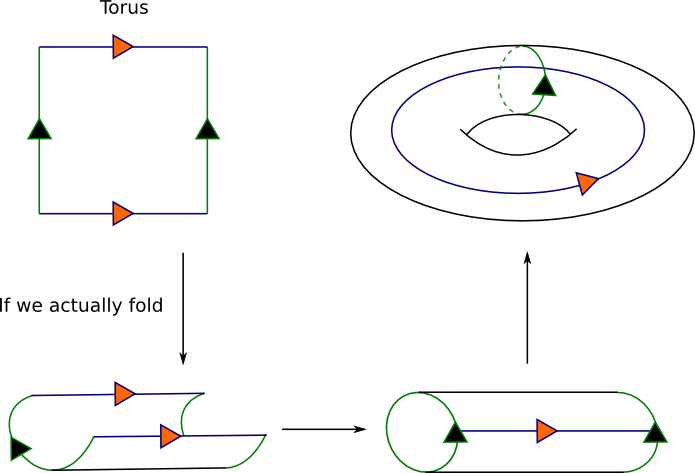
\includegraphics[height = 75mm]{toro.png}
		\caption{La costruzione del toro bidimensionale tramite quoziente.}
		\label{fig:toro}
	\end{centering}
\end{figure}